\documentclass[12pt,a4paper]{article}
\usepackage[T1]{fontenc} 
\usepackage[a4paper]{geometry}
\usepackage[brazil]{babel}
\usepackage[utf8]{inputenc}
\usepackage{setspace}
\usepackage{libertine}
 
\usepackage{url}

\usepackage{hyperref}

\usepackage{cite}  % Needed to use citations.

\usepackage{color,graphicx}
\usepackage{xcolor} 
 
\title{Visualizador de Protótipos com Realidade Virtual}
%\author{Humberto Lino Dias \\  \href{mailto:hldtux@gmail.com}{hldtux@gmail.com} }
%\author{Humberto Lino Dias \\ hldtux@gmail.com}
\author{Humberto Dias
\\Allan Tori}

 
\begin{document}
\maketitle

\abstract{O artigo apresenta um trabalho realizado na área de visualização em realidade virtual de produtos ou protótipos. Utilizamos bibliotecas em webgl \cite{github:vr_viewer_prototypes}  e Unity 5 \cite{wiki:unity} para criar dois protótipos desse visualizador. Consequentemente
este trabalho visa verificar as potencialidades e as limitações dessas ferramenta de interação gráfica
diante da complexidade dos dados que a prototipação de um produto de manufatura ou montagem
requer.}

\pagenumbering{gobble}
\singlespacing
 
 
\section{Óculos para Realidade Virtual}

\begin{center}

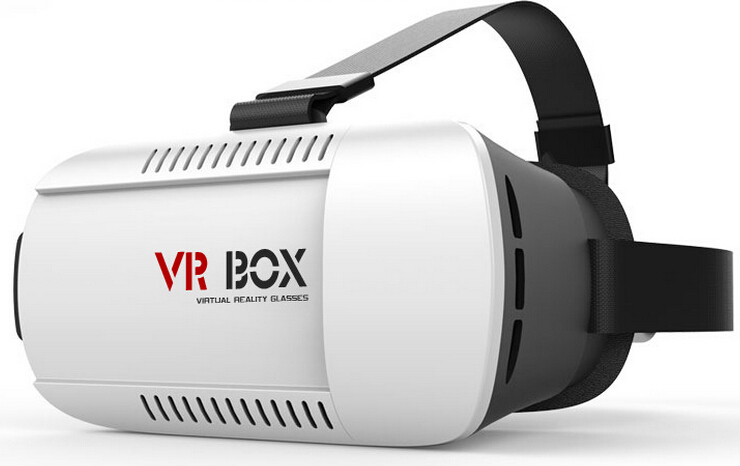
\includegraphics[height=3.1in]{vr-box-head-set.eps} \\ [1em]
\textbf{HeadSet}: VR-Box, Óculos de realidade virtual.\cite{vr_vbox_head_set}

\end{center}

 
\subsection{INTRODUÇÃO}

\paragraph{}
Atualmente as tecnologias em realidade virtual estão sendo amplamente usadas em diversas áreas do conhecimento, 
como por exemplo no design e engenharia prototipação \cite{wiki:prototipacao}, entretenimento e ciências.
No design e engenharia, a prototipação virtual é um passo importante em direção
ao desenvolvimento eficiente do produto final.
Baseados nas informações de geometria e topologia do
projeto, nos resultados da simulação obtidos por
ferramentas de modelagem combinados com os cálculos
de cinemática, o material, a tolerância e outras
informações disponíveis sobre o produto, será possível
gerar protótipos no computador para apresentações
realistas, diminuindo os custos com protótipos reais e
com o tempo de disponibilização para testes, permitindo
ainda interações com o produto até mesmo nos estágios
iniciais de desenvolvimento (Rix et al., 1995).

\paragraph{}
Pode-se utilizar a realidade virtual para desenvolver e testar um Sistema de
Intertravamento de maneira rápida para atender às necessidades deste novo mercado. A
realidade virtual é uma avançada interface homem-computador que simula um ambiente real e
permite aos participantes interagirem com o mesmo (Valério Netto, 1997). Assim com o uso da
simulação de um Sistema de Intertravamento em ambiente de realidade virtual, cria-se um
protótipo virtual de um sistema, reduzindo-se os custos e o tempo de desenvolvimento deste
Sistema, uma vez que são eliminados etapas de confecção de protótipos físicos, bem como
proporciona-se uma melhoria da qualidade do produto, pois a aplicação de diferentes
alternativas do projeto pode ser realizada mais rapidamente, permitindo uma melhoria da
validação das soluções apropriadas que satisfaça os parâmetros especificados para o sistema,
com um menor custo. Podemos dizer que realidade virtual (RV) \cite{wiki:virtual_reality} é a forma mais avançada de interface entre o usuário e o computador até agora disponível
(HANCOCK, 1995). Trata-se de uma interface homem-máquina que simula um ambiente real e
permite aos participantes interagirem com o mesmo (LATTA \& OBERG, 1994). 


\subsection{VISÃO GERAL DO PROJETO PRÁTICO}
\paragraph{}
No projeto aqui apresentado, foram feitos dois protótipos de simuladores em realidade virtual. No primeiro foi utilizado a biblioteca ‘‘Three.js’’ \cite{wiki:threejs} e a plataforma é web, portanto foi necessário um importador de objetos Javascript ( JSON ) \cite{wiki:json} para os objetos 3D, também em JSON \cite{wiki:json}. Nesse primeiro protótipo, houve uma dificuldade em se
criar uma interface, pois seria necessário recriar mecânicas de raycast para conseguir captar para onde o usuário está olhando. No segundo protótipo utilizamos a engine de jogos Unity \cite{wiki.city} 5.0, uma biblioteca de importação de objetos em obj e outra biblioteca para acessar os arquivos do computador ou celular gerando um ‘‘path’’  para a biblioteca de importação. No Unity \cite{wiki:unity}, a mecânica de raycast já é bem implementada
,portanto não houve dificuldade de se criar uma interface interativa. 

\paragraph{}

\subsection{CONCLUSÕES}
\paragraph{}
Neste projeto percebe-se a grande difereça entre visualizar um protótipo de um software 3d num monitor e o mesmo protótipo visualizado em realidade virtual.
Segundo Kirner(1996), a grande vantagem desse tipo de interface em RV \cite{wiki:virtual_reality}  é
que o conhecimento intuitivo do usuário a respeito do mundo físico pode ser transferido para manipular o mundo virtual. O usuário entra no espaço virtual das aplicações e visualiza,
manipula e explora os dados da aplicação em tempo real, usando seus sentidos, particularmente os movimentos naturais tridimensionais do corpo. Para apoiar esse tipo de interação, o
usuário utiliza dispositivos não convencionais como capacete de visualização e controle, luvas e outros. Estes dispositivos dão ao usuário a impressão de que a aplicação está funcionando
no ambiente tridimensional real, permitindo sua exploração a movimentação natural dos objetos com o uso das mãos.

\newpage
\section{Apêndice}

Por fim, a referência do aplicativo na PlayStore e video sobre este trabalho:

\begin{enumerate}
\item  \url{https://play.google.com/store/apps/details?id=br.vr.viewer.models} \cite{playstore:app_vr_viewer_prototypes}
\item  \url{https://youtu.be/jAuvG02FWO8} \cite{youtube:app_vr_viewer_prototypes}
\end{enumerate}


\bibliography{refs}
\bibliographystyle{plain}
 
\end{document}